\section{Other Factors}
\subsection{Temperature}\label{D_vs_temp}
For SiC divacancies ($S=1$) the ZFS parameter $E$ shows no dependence on temperature. However, the ZFS parameter $D$ varies with temperature.

$D$ has been measured for both the PL5 and PL6 defects in SiC from close to $0$K to around $550$K and the dependence of $D$ has been fitted to the change in temperature.
Both defects show an approximately linear relationship near room temperature which is shown in Figure \ref{fig:PL5PL6DvsT}.


\td{Font size}
\begin{figure}[H]
	\begin{center}
		% \missingfigure{Plot of both the PL5 and PL6 temperature dependence from 0 to 550K, specifically highlighting the linear region. }
		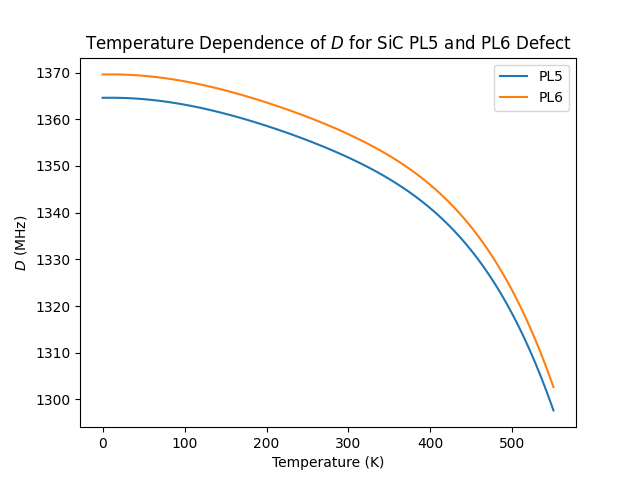
\includegraphics[width=0.49\textwidth]{figures/SiC-PL5PL6-D(T).png}
		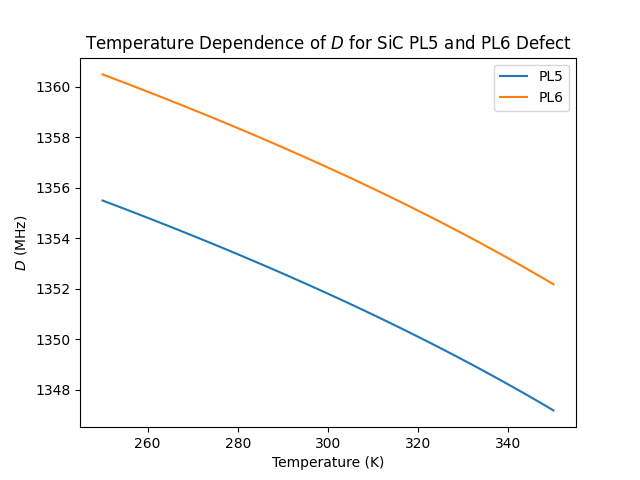
\includegraphics[width=0.49\textwidth]{figures/SiC-PL5PL6-D(T)-close.png}
		\caption{ZFS parameter $D$ temperature dependence for the PL5 and PL6 $S=1$ defect in SiC from 0-550 K (left) and 250-350 K (right). }\label{fig:PL5PL6DvsT}
	\end{center}
\end{figure}

\td{Update the T dependence of PL5 and PL6 and regen the figure. Also update temp linear range in figure caption.}

This allows for the consideration of the system temperature, enabling sensing at a range of temperatures. Additionally, if other parameters are well known, the system may be used as a thermometer.

% \section{Strain and Pressure}
\subsection{Strain}
% {\color{red}
% Two physical effects contribute to stark parameters $d_\parallel$ and $d_\perp$. 
% Electric fields distort the positions of atoms in the SiC lattice neighboring
% the divacancy and electric fields shift the electron
% distribution surrounding the defect. Although these effects
% occur simultaneously and cannot be distinguished by
% experiments alone,
% }
Strain, which alters the $D$ and $E$ parameters due to a distribution in the ligand field \cite{Jeschke} will influence the Hamiltonian, specifically the zero field splitting of the spin system. Using the same reasoning as
in section \ref{stark}, we could derive a strain Hamiltonian which is identical to \eqref{eq:stark_hamiltonian}.
Therefore, exactly as we consider the "whole effect" of the contributions to the zero field Hamiltonian, we consider
the combined effect of strain and applied $\vec{E}$. Put simply, \index{strain}{strain} is treated as an effective electric
field \cite{PhysRevLett.112.187601}.

An application of this duality, is that we may use $\vec{E}$ measuring techniques in shielded environment to determine strain.

% [32] A. E. Hughes and W. A. Runciman, Proceedings of the
% Physical Society 90, 827 (1967).
% [33] G. Davies and M. F. Hamer, Proceedings of the Royal
% Society A: Mathematical, Physical and Engineering Sci-
% ences 348, 285 (1976)

% \begin{figure}[H]
% 	\begin{center}
% 		% \includegraphics[width=0.95\textwidth]{figures/}
% 		\missingfigure{Figure illustrating how strain is an effective electric field}
% 	\end{center}
% 	\caption{\td{write caption}}\label{fig:}
% \end{figure}

\subsection{Pressure}
The effect of \index{pressure}{pressure} has been studied for SiC divacancies. The zero field splitting parameter $D$ shows
a linear dependence on pressure up to $40$ GPa \cite{doi:10.1021/acs.nanolett.2c03378} and is shown in figure \ref{fig:pressure_d}.

\begin{figure}[H]
	\begin{center}
		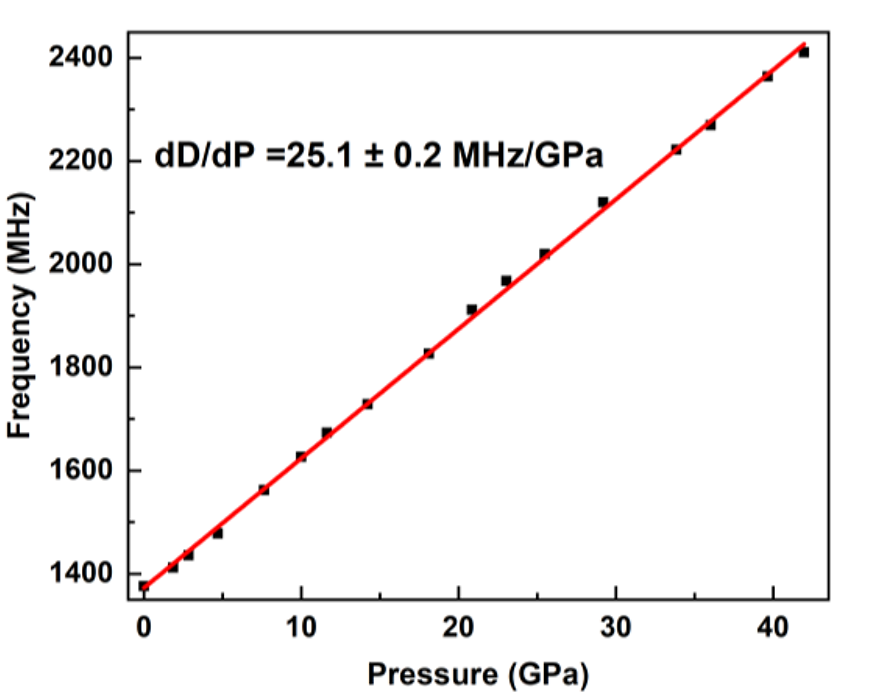
\includegraphics[width=0.6\textwidth]{figures/PressureDependence.png}
		% \missingfigure{Figure illustrating how pressure is an effective magnetic field}
	\end{center}
	\caption{Linear dependence of zero field parameter D to applied pressure as shown in the work by Liu et al.}\label{fig:pressure_d}
\end{figure}

This allows for the consideration of the pressure applied to the system which allows for sensing in environments above ambient pressure. Additionally, if other parameters are held constant or the sensor is designed such that they cannot contribute (e.g. electro-magnetic shielding) the system can be utilised as a pressure gauge.

% \cite{PhysRevLett.112.087601}

